En la figura \ref{fig:con_paralelizacion_datos} se presenta la misma
aplicación (esta vez se la denomina \textit{app}). En este ejemplo
los datos representados por $D$ anteriomente, se
dividien en $D_{n}$ secciones más pequeñas que son distribuidas a distintos
núcleos de procesamiento \footnote{en el ejemplo se utilizan 4, aunque pueden ser más
núcleos dentro de un procesador}. Una copia idéntica de la aplicación (Figura
\ref{fig:sin_paralelizacion_datos}) se encuentra corriendo en cada uno de los
cuatro núcleos del ordenador, cada una de estas copias idénticas se
encuentra trabajando con datos distintos (ya que a cada una de las copias le
toca una sección $D_{n}$ diferente).

\begin{figure}[h]
  \centering
  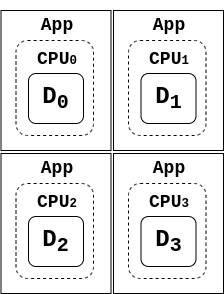
\includegraphics[width=0.3\linewidth]{figuras/procesamiento_paralelo_con_paralelizacion_datos.png}
  \caption{Aplicación con paralelización de datos}
  \label{fig:con_paralelizacion_datos}
\end{figure}

Una interpretación alternativa se puede ver en la figura
\ref{fig:con_paralelizacion_datos_alt}, este gráfíco se puede leer como ``Una
aplicación que se encuentra corriendo sobre distintos nucleos, con distintos
fragmentos de los datos originales''

\begin{figure}[h]
  \centering
  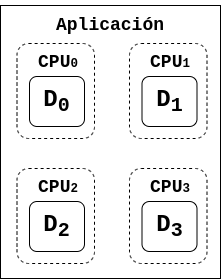
\includegraphics[width=0.3\linewidth]{figuras/procesamiento_paralelo_con_paralelizacion_datos_alt.png}
  \caption{Aplicación con paralelización de datos - Representación alternativa}
  \label{fig:con_paralelizacion_datos_alt}
\end{figure}
